\documentclass[a4paper]{article}
\usepackage{url}
\usepackage[super]{nth}
\usepackage{color}
\usepackage{colortbl}
\usepackage[table]{xcolor}  % 
\definecolor{gray}      {gray}  {0.749}
\definecolor{lgray}     {gray}  {0.85}
\definecolor{red}       {rgb}   {1 ,  0  , 0}
\definecolor{green}     {rgb}   {0 ,  1  , 0}
\definecolor{blue}      {rgb}   {0 ,  0  , 1}
\definecolor{darkgreen} {rgb}   {0 , 0.6 , 0}
\usepackage{longtable}
\usepackage{multirow}
\newenvironment{zebratabular}{\rowcolors{2}{lgray}{white}\tabular}{\endtabular}
\newenvironment{zebralongtable}{\rowcolors{2}{lgray}{white}\longtable}{\endlongtable}
\usepackage{fancyhdr}
\pagestyle{fancy}
\fancyhf{}
\fancyhead[L]{EENG - Handout}
\fancyhead[C]{Lucerne University of Applied Sciences and Arts\\Engineering \& Architecture}
\fancyhead[R]{Manuel Cortez\\Sandro Wicki\\Daniel Winz}
\fancyfoot[L]{\today}
\fancyfoot[C]{}
\fancyfoot[R]{\thepage}
\renewcommand{\headrulewidth}{0.4pt}
\renewcommand{\footrulewidth}{0.4pt}

\title{Production of an electronic device - Fire detector}
\author{Manuel Cortez\\Sandro Wicki\\Daniel Winz}
\date{\today}

\begin{document}
\maketitle

\section{Summary}
Possible signs for a fire to detect are heat, smoke and light. For all of 
those a specific type of fire detector exists. Detectors can use a single 
sensor or a combination of sensors to detect fires and suppress false alarms. 
The detectors are connected to the panel via a two wire bus with a ring 
topology. Therefore in case of a short circuit the whole system remains 
active. In the model used as example the configuration can be changed wireless. 
Then the communication is based on radio frequency and light. 
\begin{wrapfigure}{R}{0.5\textwidth}
\centering
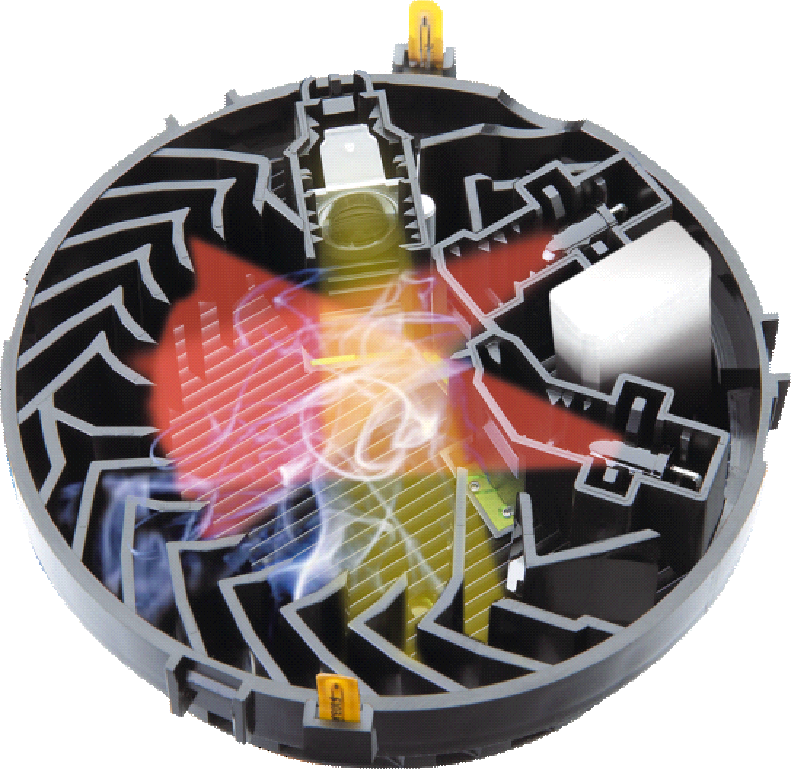
\includegraphics[width=0.5\textwidth]{det_int.png}
\caption{Interior of a fire detector with temperature sensors (yellow spots), 
    optical sensors (red and yellow beams) and gas sensor(white block)}
\label{fig:det_int}
\end{wrapfigure}

The printed circuit board (PCB) is based on glass fibre reinforced resin. This 
is coated with a thin layer of copper. The traces are structured via etching. 
The structured PCB ist then coated with green solder stop. This reduces the 
risk of short circuit in the soldering process. The PCB can be labeled with a 
white silk screen to mark component positions or add notes or component 
designators. When the PCB is completed, the components can be soldered. 
Therefore the components are placed in an automated pick and place machine 
after solder paste has been applied. The soldering process is performed in 
an oven where the solder paste is heated above its melting temperature. 

The fire detector is designed to be mounted on the ceiling. So the mechanical 
strength of the material is not the most important requirement. As fire 
detectors are used in big quantities, it is necessary to produce them as 
cheaply as possible. One possible way is to use injection moulding for the 
production process. Granules made of thermoplastics will be injected with 
pressures of up to 2500 bar into a form. The pressure is necessary to assure 
that the entire mould is filled out.  


\section{Word bank}
\begin{zebratabular}{p{0.3\textwidth}p{0.65\textwidth}}
    \rowcolor{gray} Word &
        Definition\\
\end{zebratabular}


\section{Guiding questions}
\begin{enumerate}
    \item What are the signs for a fire? 
    \begin{itemize}
        \item Heat
        \item Smoke
        \item Light
    \end{itemize}
    \item What happens when the cables are not connected anymore?
    \item How can the microprocessor save energy?
    \item What kind of detection techniques exist?
    \item What is a suitable way of producing the case of the detector?
    \item How does the sensor react to inputs?
    \item What is the paradoxon of producing the case?
\end{enumerate}


\section{References}
\begin{itemize}
    \item Siemens document
\end{itemize}
\end{document}
